\documentclass[11pt,a4paper]{article}

\usepackage[margin=2.2cm]{geometry}
\usepackage[T1]{fontenc}
\usepackage{lmodern}
\usepackage{amsmath,amssymb}
\usepackage{graphicx}
\usepackage{booktabs}
\usepackage{tabularx}
\usepackage{array}
\usepackage{float}
\usepackage{needspace}
\usepackage{caption}
\usepackage{enumitem}
\usepackage{xcolor}
\usepackage{algorithm}
\usepackage{algpseudocode}
\usepackage[hidelinks]{hyperref}

\graphicspath{{figures/}}
\setlist{itemsep=2pt,topsep=4pt}
\captionsetup{font=small,labelfont=bf}
\newcommand{\ours}[1]{\textcolor[HTML]{1B7F5A}{#1}}

\newcommand{\fppvsMinAcc}{81.3}
\newcommand{\fppvsMaxAcc}{99.6}
\newcommand{\fppvsMeanAcc}{92.8}
\newcommand{\fppvsWorstScenario}{Metro 1}
\newcommand{\fppvsLowestRun}{77.5}
\newcommand{\trainSeconds}{72}
\newcommand{\numSeeds}{5}
\newcommand{\origMinAcc}{43.6}
\newcommand{\origMaxAcc}{64.6}
\newcommand{\origMeanAcc}{54.1}
\newcommand{\origGainMin}{31.5}
\newcommand{\origGainMax}{47.1}
\newcommand{\origGainMean}{38.7}
\newcommand{\zhangMinAcc}{44.5}
\newcommand{\zhangMaxAcc}{74.0}
\newcommand{\zhangMeanAcc}{57.3}
\newcommand{\zhangGainMean}{35.5}

\title{\textbf{Fairness-aware and Parallelized SFC Placement with VNF Sharing:\\
Implementation, Limitations and Modifications}\\[4pt]
\large Advanced Computer Networks -- Project Report}
\author{23CSB0B03 \quad 23CSB0B17 \quad 23CSB0B23 \quad 23CSB0B56}
\date{}

\begin{document}
\maketitle

\begin{abstract}
We studied FPPVS, a framework by Zhu, Li and Rezaeipanah~\cite{fppvs} that places
service function chains (SFCs) in MEC-enabled IoT networks using SFC
parallelization, VNF sharing, fairness-aware allocation and federated deep
reinforcement learning (FDRL). We built a full Python implementation of it. Our
first version accepted only about 10\% of requests, worse than a random
placement. We traced this to several gaps in the problem as it was specified
and in our implementation, and then changed the formulation and the algorithm:
Poisson arrivals at a stated offered load, a placement mask that checks compute,
bandwidth and latency before a data center is chosen, a per-data-center actor
network with a placement prior, honest accounting for shared VNF instances,
rollback-and-retry admission, and corrected federated training. On synthetic
Backbone (24 nodes) and Metro (17 nodes) topologies at three load levels, the
updated FPPVS accepts between \fppvsMinAcc\% and \fppvsMaxAcc\% of requests on
a hold-out stream (mean of \numSeeds{} seeds), and it holds less bandwidth per
running SFC than every other method. Under the same conditions, the original
FPPVS as specified in the paper accepts \origMinAcc--\origMaxAcc\%, a 2022
SFC-placement method by Zhang et al.\ accepts \zhangMinAcc--\zhangMaxAcc\%, and
greedy and random placement stay between 52\% and 73\%.
\end{abstract}

\noindent\textbf{How to read this report.} Material that describes the original
paper is written as ``the paper'' or ``the original work''. Everything our team
designed, changed or measured is marked as ours and is summarised in
Table~\ref{tab:contrib}.

%=====================================================================
\section{Introduction}
%=====================================================================

\subsection{Problem addressed}
Network Function Virtualization (NFV) replaces dedicated middleboxes, such as
firewalls (FW), intrusion detection (IDS), deep packet inspection (DPI), load
balancers (LB) and NAT, with software Virtual Network Functions (VNFs). A
network service is an ordered list of VNFs called a Service Function Chain
(SFC). In a Mobile Edge Computing (MEC) network the VNFs run on small edge data
centers (DCs) that have limited compute, and the DCs are connected by links with
limited bandwidth and non-zero latency. The \emph{SFC placement problem} asks,
for every arriving request, on which DC each VNF should run and how traffic
should be routed between them, so that capacity, bandwidth and the request's
latency limit are respected. The problem is NP-hard and has to be solved online,
because requests arrive one after another and leave after their lifetime.

\subsection{Motivation}
Two effects make the problem harder in IoT/MEC settings. First, end-to-end
latency grows with chain length when every packet passes through every VNF in
sequence. Second, many requests compete for the same small edge DCs, so a
placement policy that only looks at the current request can starve later ones.
Existing methods tend to address only one of these at a time: network function
parallelism reduces latency, while VNF reuse reduces resource use. Fairness
between competing flows is usually ignored.

\subsection{Main contributions of the original paper}
The paper~\cite{fppvs} proposes FPPVS, which combines four ideas:
\begin{enumerate}
  \item \textbf{SFC parallelization (Algorithm 1).} VNFs are split into
  \emph{shapers}, which modify packets and must stay in order, and
  \emph{monitors}, which only read packets. Monitors are moved onto branches
  that run in parallel with the main chain, and a dependency matrix says where
  each branch must rejoin. The sequential SFC (s-SFC) becomes a directed acyclic
  graph (p-SFC), and latency is measured on its critical path.
  \item \textbf{VNF sharing with demand prediction.} Before creating a new VNF
  instance, the method tries to reuse a compatible live instance. A bounded
  SFC queue network (SQN) and an LSTM forecast upcoming demand per VNF type.
  \item \textbf{Fairness-aware allocation.} A concave $\alpha$-fair utility over
  flow throughput is part of the objective, so a few heavy flows cannot take all
  the resources. Jain's fairness index (JFI) is reported.
  \item \textbf{Federated actor-critic learning.} Local agents with a CNN
  actor-critic place VNFs, and a cloud server combines their models with
  federated averaging (FedAvg)~\cite{fedavg}. Exploration uses a reward-driven
  adaptive $\epsilon$-greedy rule.
\end{enumerate}
The paper reports 88.1\% service acceptance on a backbone topology and 75.9\% on
a metropolitan topology, ahead of four baselines (RVNF, DRL-SFCP, PVFP and DPC).

%=====================================================================
\section{Limitations of the Original Work}
%=====================================================================

We list the limitations we found while implementing the paper. Some are gaps in
what the paper specifies, so it cannot be reproduced exactly. Others are design
problems that showed up once the method ran. Table~\ref{tab:limits} states which
ones our project addresses.

\begin{enumerate}[label=\textbf{L\arabic*.}]
  \item \textbf{The workload is under-specified.} The paper fixes a mean
  service lifetime of 1000 time units and 4000 requests, but it does not give
  the arrival rate. The arrival rate decides how many SFCs are active at the
  same time, and so it decides the acceptance ratio. When we used one arrival
  per time unit, about 1000 SFCs would have to be active at once, while a
  24-node network with 10--20 compute units per DC can only hold about 70--100.
  \item \textbf{Datasets and code are not available.} The USAnet and Italian
  operator topologies, the traffic traces, the MATLAB code and the baseline
  configurations are not published. Results can only be compared in spirit.
  \item \textbf{Feasibility is checked too late.} The paper prunes nodes that
  lack compute, but bandwidth and the latency limit are checked only after the
  whole chain is placed. An agent can therefore spend a full episode building a
  placement that is rejected at the last step.
  \item \textbf{The sharing model can overbook capacity.} The paper does not say
  how much capacity a shared instance reserves or when it is released. A natural
  reading, which our first version followed (instances sized at three times the
  demand, only one times reserved), lets the pool use capacity that the DC does
  not have.
  \item \textbf{The CNN cannot tell data centers apart.} The paper's actor is a
  CNN over a feature grid followed by fully connected layers, with one output per
  DC. After global pooling, the network no longer knows which column belongs to
  which DC, so it can only learn fixed DC preferences.
  \item \textbf{Each episode is one request.} The reward only sees the current
  request. Effects on later requests, such as fragmentation or a saturated link,
  reach the agent only indirectly.
  \item \textbf{Resource efficiency is reported only as utilization.} Higher
  utilization can mean better packing, but it can also mean more waste per
  request. The paper does not report resources held per served SFC over time.
\end{enumerate}

\begin{table}[H]
\centering\small
\caption{Limitations and how our project treats them.}
\label{tab:limits}
\begin{tabularx}{\linewidth}{l X l}
\toprule
 & Our treatment & Status \\
\midrule
L1 & Poisson arrivals whose rate is set from an explicit offered load $\rho$ & \ours{Addressed} \\
L2 & Synthetic graphs of the same size; simple, documented baselines & Partly (data still missing) \\
L3 & Look-ahead mask on compute, every routed link and the latency bound & \ours{Addressed} \\
L4 & Per-instance overhead model, all usage counted against physical capacity & \ours{Addressed} \\
L5 & Per-column actor with shared weights plus a learnable placement prior & \ours{Addressed} \\
L6 & Placement prior with future-hop term; rollback-and-retry admission & Partly \\
L7 & New metrics: resources held per running SFC and resource-time per accepted SFC & \ours{Addressed} \\
\bottomrule
\end{tabularx}
\end{table}

\paragraph{Problems in our first implementation.} Before the modifications, our
implementation of the paper had its own bugs. The package did not import (a
queue-memory class had been deleted), training crashed when every action was
masked, federated agents replayed the same ten requests in every round and
shared one resource ledger, and the state ignored resources held by earlier
requests. With these bugs and limitations L1--L5, it accepted
10.4\% of requests, less than greedy (15.8\%) and random (11.6\%) placement. A
diagnosis run showed that every rejection was due to link bandwidth running out.

%=====================================================================
\section{System Model and Architecture}
%=====================================================================

\subsection{Substrate network}
The MEC network is an undirected graph $G_s=(V_s,E_s)$. Each DC
$v_i\in V_s$ has compute capacity $C_i$. Each link $(v_i,v_j)\in E_s$ has
latency $L_{ij}$ and bandwidth capacity $B_{ij}$. Traffic between two DCs follows
the latency-shortest path $P(v_i,v_j)$. Two VNFs on the same DC exchange traffic
at no bandwidth or network latency cost. We use two topologies with the sizes
used in the paper: \emph{Backbone} (24 DCs, 47 links, like USAnet) and
\emph{Metro} (17 DCs, 29 links, like the Italian access network).

\subsection{Requests supported}
A request $u$ is the tuple
$(s_u, \mathcal{F}_u, d_u, D_u, t_u, \tau_u, r_u, L^{\max}_u)$: source DC,
ordered VNF list, destination DC, dependency matrix, arrival time, lifetime
(TTL), data rate and maximum end-to-end latency. Each VNF $f\in\mathcal{F}_u$
has a type, a kind (shaper or monitor), a compute demand $c_f$ and a processing
latency $\ell_f$. The implementation supports:
\begin{itemize}
  \item \textbf{Five VNF types}: IDS, DPI, LB, FW and NAT. IDS and DPI can act
  as monitors; the others are shapers.
  \item \textbf{Purely sequential chains} (only shapers), \textbf{purely
  parallel chains} (only monitors, all branching from the source), and
  \textbf{mixed chains} in which a monitor must finish before a later shaper.
  \item \textbf{Chains of 4 to 10 VNFs} with heterogeneous compute demand and a
  heavy-tailed (power-law) data rate.
\end{itemize}

For each request the system outputs: an accept/reject decision; if accepted, the
DC for every VNF, the substrate route of every virtual link, the latency split
into network, virtualization and processing parts on the critical path, the
compute and bandwidth reserved, and which VNF instances were reused or started.
If rejected, it outputs the reason (for example, no DC fits the next VNF).

\subsection{Architecture}
Figure~\ref{fig:arch} shows the components. Blue blocks follow the paper
directly, orange blocks are paper ideas that we re-implemented, and green blocks
are new or changed by our team.

\begin{figure}[H]
\centering
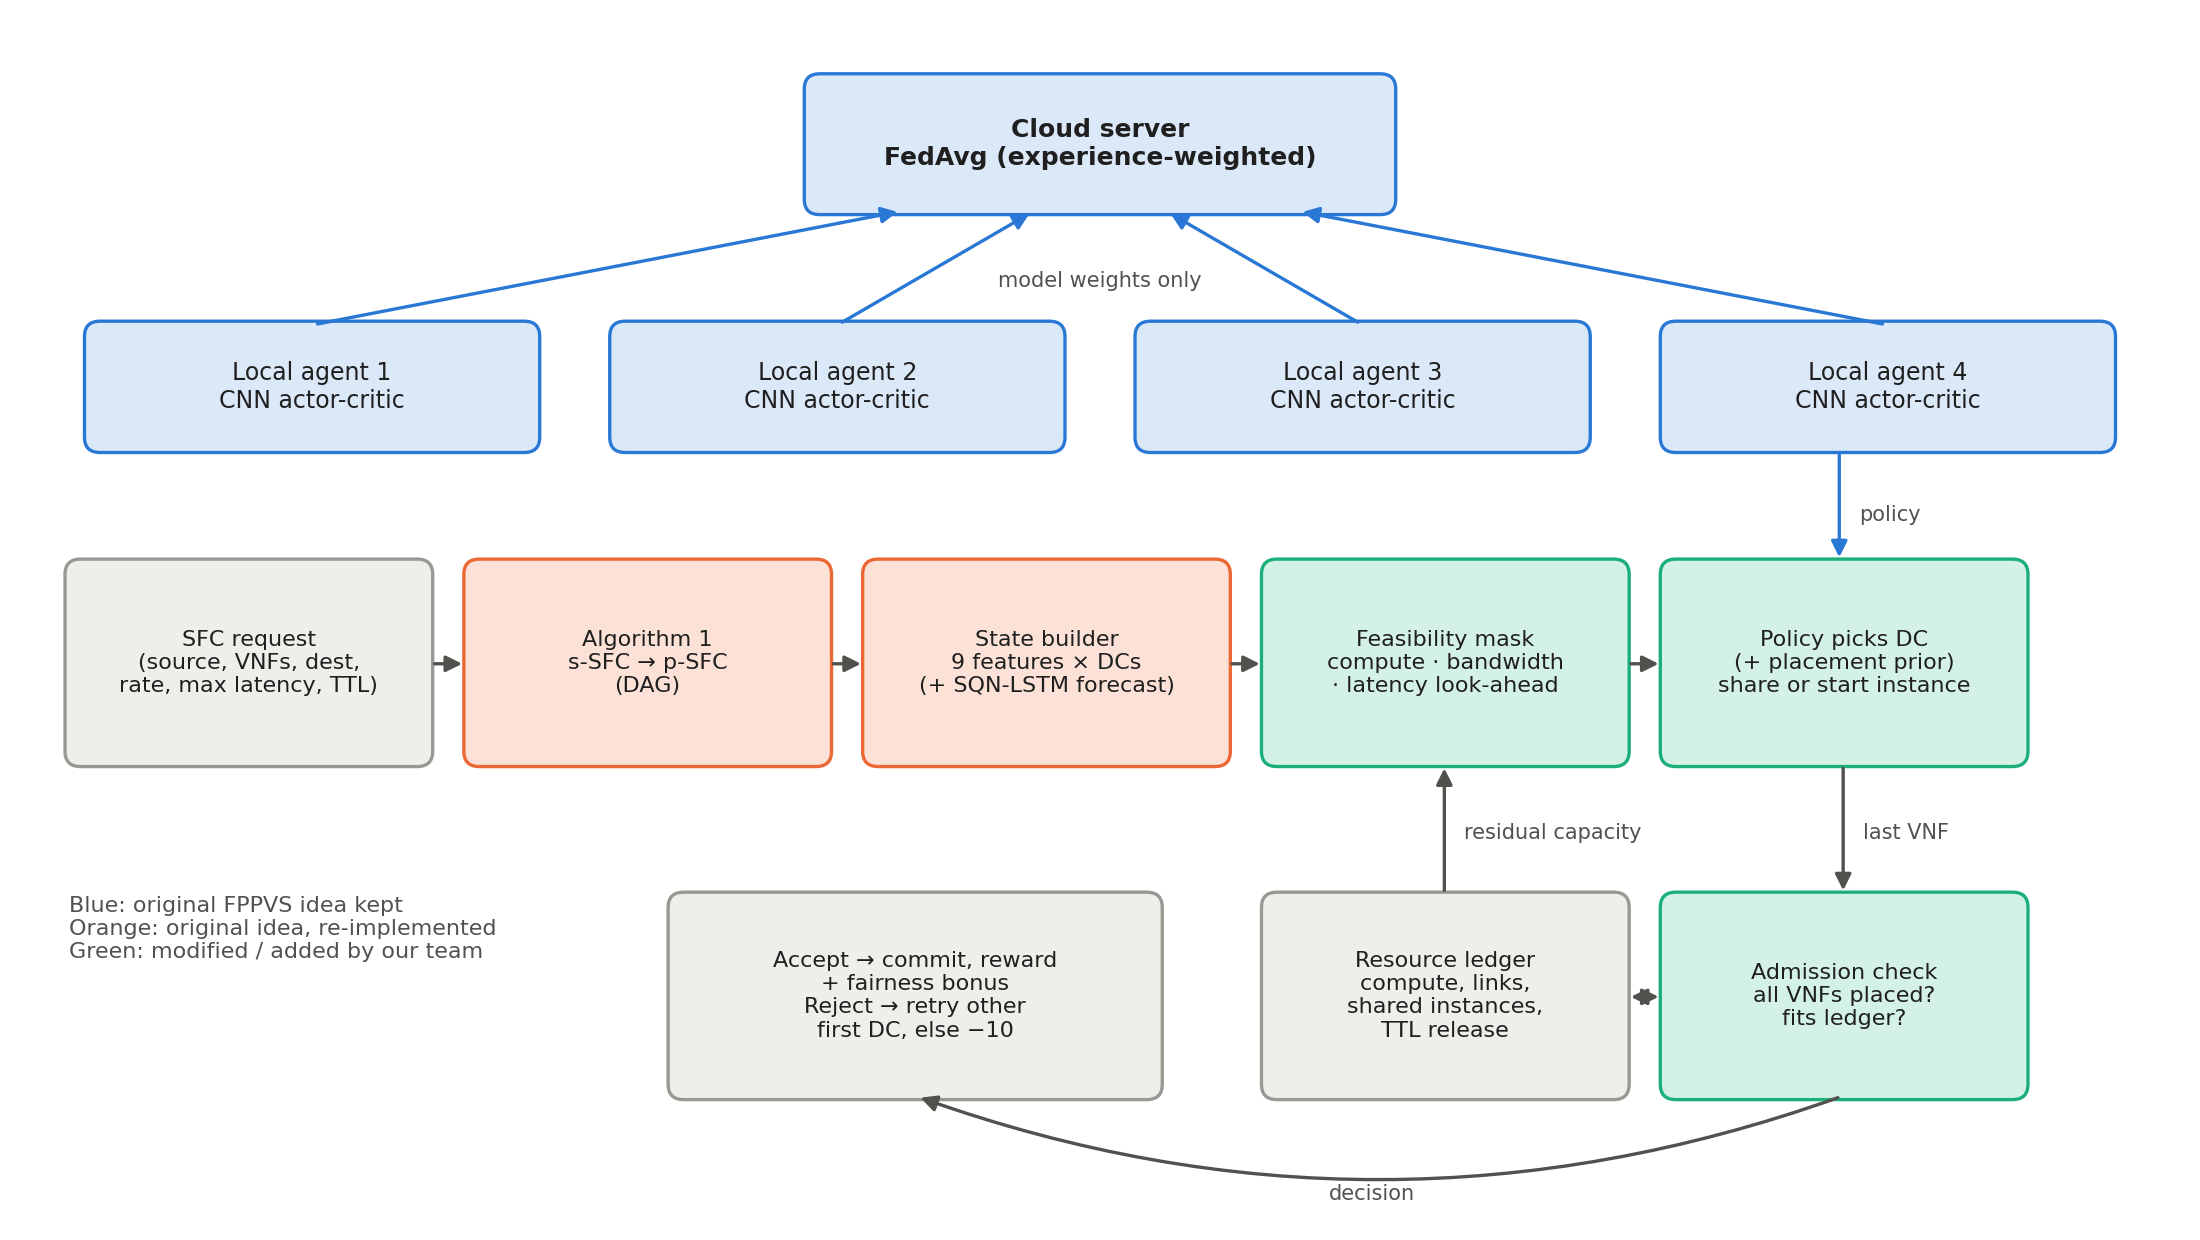
\includegraphics[width=\linewidth]{architecture.png}
\caption{System architecture. A request is converted to a p-SFC, its VNFs are
placed one at a time by a local agent under a feasibility mask, and the
admission check commits or rejects the whole chain against the resource ledger.
Agents share model weights through FedAvg, never raw request data.}
\label{fig:arch}
\end{figure}

\begin{itemize}
  \item \textbf{Algorithm 1 (s-SFC to p-SFC).} Figure~\ref{fig:psfc} shows the
  output of our implementation for a five-VNF chain. FW, NAT and LB stay on the
  main chain. IDS branches off after FW and must rejoin before NAT because the
  dependency matrix says so. DPI has no dependent shaper, so it rejoins at the
  destination.
  \item \textbf{State builder and SQN-LSTM.} Builds a grid with one column per DC
  and nine feature rows (Section~\ref{sec:approach}). The SQN keeps the per-type
  demand of the last five requests, and the LSTM predicts the next one.
  \item \textbf{Feasibility mask, policy and admission} are described in
  Section~\ref{sec:approach}.
  \item \textbf{Resource ledger.} Holds the compute, link bandwidth and live
  shared instances of all active SFCs, releases them when a TTL expires, and
  integrates resource use over time for the metrics.
  \item \textbf{Federated learning.} Four local agents, each with its own request
  stream and ledger, train locally; the cloud averages their weights.
\end{itemize}

\begin{figure}[H]
\centering
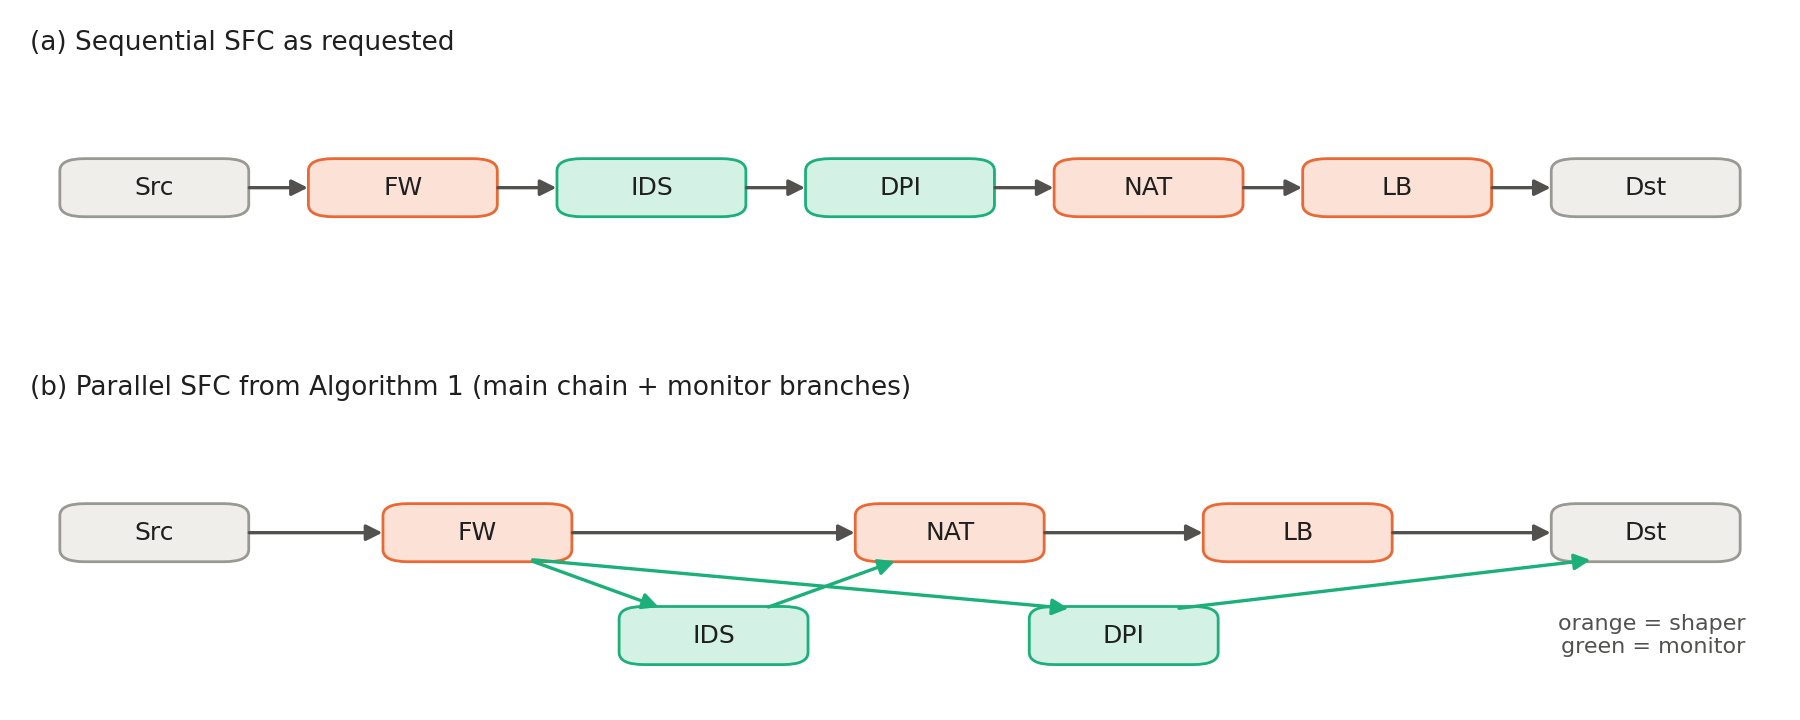
\includegraphics[width=0.9\linewidth]{psfc-example.png}
\caption{Algorithm 1 as implemented. Top: requested sequential chain.
Bottom: generated p-SFC. IDS must finish before NAT; DPI has no dependent
shaper and rejoins at the destination.}
\label{fig:psfc}
\end{figure}

%=====================================================================
\section{Modified Problem Formulation}
%=====================================================================

\subsection{Original formulation (paper)}
The paper minimizes a weighted sum over time,
\begin{equation}
F_{obj} = \min \sum_{t} \xi_{cost} O_{cost}(t) + \xi_{E2E} O_{E2E}(t)
 - \xi_{acc} O_{acc}(t) - \xi_{utility} O_{utility}(t),
\end{equation}
where $O_{acc}=\frac{1}{|U|}\sum_u y_u$ is the acceptance ratio ($y_u=1$ if
request $u$ is accepted), $O_{cost}$ is deployment cost, $O_{E2E}$ is end-to-end
latency and $O_{utility}$ is the $\alpha$-fair throughput utility. Constraints
cover DC capacity, link bandwidth, latency, placement uniqueness and VNF
dependencies.

\subsection{Our modifications}

\paragraph{M1. Explicit offered load (L1).} Requests arrive as a Poisson process
with rate $\lambda$, and lifetimes are exponential with mean $\bar\tau=1000$. We
set $\lambda$ from a target offered load
\begin{equation}
\rho = \frac{\lambda\,\bar\tau\,\bar c}{\sum_{i} C_i},
\qquad \bar c = 7\times 0.7 = 4.9,
\end{equation}
where $\bar c$ is the mean compute demand of one SFC (4--10 VNFs of
0.5--0.9 units each). $\rho=1$ means the average offered compute equals the
total compute of the network. We evaluate $\rho\in\{0.5, 0.75, 1.0\}$ and use
$\rho\in\{1.25, 1.5\}$ as overload stress tests.

\paragraph{M2. Instance-based compute model (L4).} Each live VNF instance costs a
fixed overhead $o$ (its VM or container footprint, $o=0.25$) plus the demand of
every flow it serves. Let $\mathcal{A}(t)$ be the set of active requests and
$\mathcal{I}_i(t)$ the set of live instances on DC $v_i$. The compute
constraint is
\begin{equation}
\sum_{u\in\mathcal{A}(t)} \sum_{f\in\mathcal{F}_u} c_f\, x^u_{f,i}
\;+\; o\,|\mathcal{I}_i(t)| \;\le\; C_i \qquad \forall v_i, t,
\end{equation}
where $x^u_{f,i}=1$ if VNF $f$ of request $u$ runs on $v_i$. With sharing, an
instance of type $k$ on $v_i$ is created by the first VNF of that type and
removed when its last user leaves. Without sharing, every VNF has its own
instance.

\paragraph{M3. Bandwidth and latency on the p-SFC.} For every virtual edge
$(a,b)$ of the p-SFC, the data rate $r_u$ is reserved on each link of
$P(\pi(a),\pi(b))$, where $\pi$ is the placement:
\begin{equation}
\sum_{u\in\mathcal{A}(t)} \sum_{(a,b)\in E_u} r_u\,
\mathbb{1}\big[(v_i,v_j)\in P(\pi(a),\pi(b))\big] \le B_{ij}.
\end{equation}
The latency of a request is the longest source-to-destination path in the
p-SFC, counting link latency and VNF processing:
$L_u = \max_{p} \sum_{(a,b)\in p} \big(L_{P(\pi(a),\pi(b))} + \ell_b\big)
\le L^{\max}_u$.

\paragraph{M4. Objective.} The main objective stays the same as the paper:
maximize $O_{acc}$. As a second objective we minimize the resources held per
served request over time (L7):
\begin{equation}
R_{comp} = \frac{\int_t \sum_i \mathrm{used}_i(t)\,dt}{\#\text{accepted}},
\qquad
R_{bw} = \frac{\int_t \sum_{(i,j)} \mathrm{used}_{ij}(t)\,dt}{\#\text{accepted}}.
\end{equation}
Latency and fairness enter through the reward (Section~\ref{sec:reward}), as in
the paper. We do not model monetary cost separately, because with a fixed price
per unit it is proportional to $R_{comp}$.

%=====================================================================
\section{Proposed Approach}\label{sec:approach}
%=====================================================================

\subsection{Overview}
Each request is one episode. Its VNFs are placed one at a time in their original
order, which is also a topological order of the p-SFC. When VNF $f$ is placed on
a candidate DC, every virtual edge that enters $f$ (and its edge to the
destination, if it has one) can already be routed. This is what makes an early
feasibility check possible. Figure~\ref{fig:flow} and Algorithm~\ref{alg:place}
show one decision.

\begin{figure}[H]
\centering
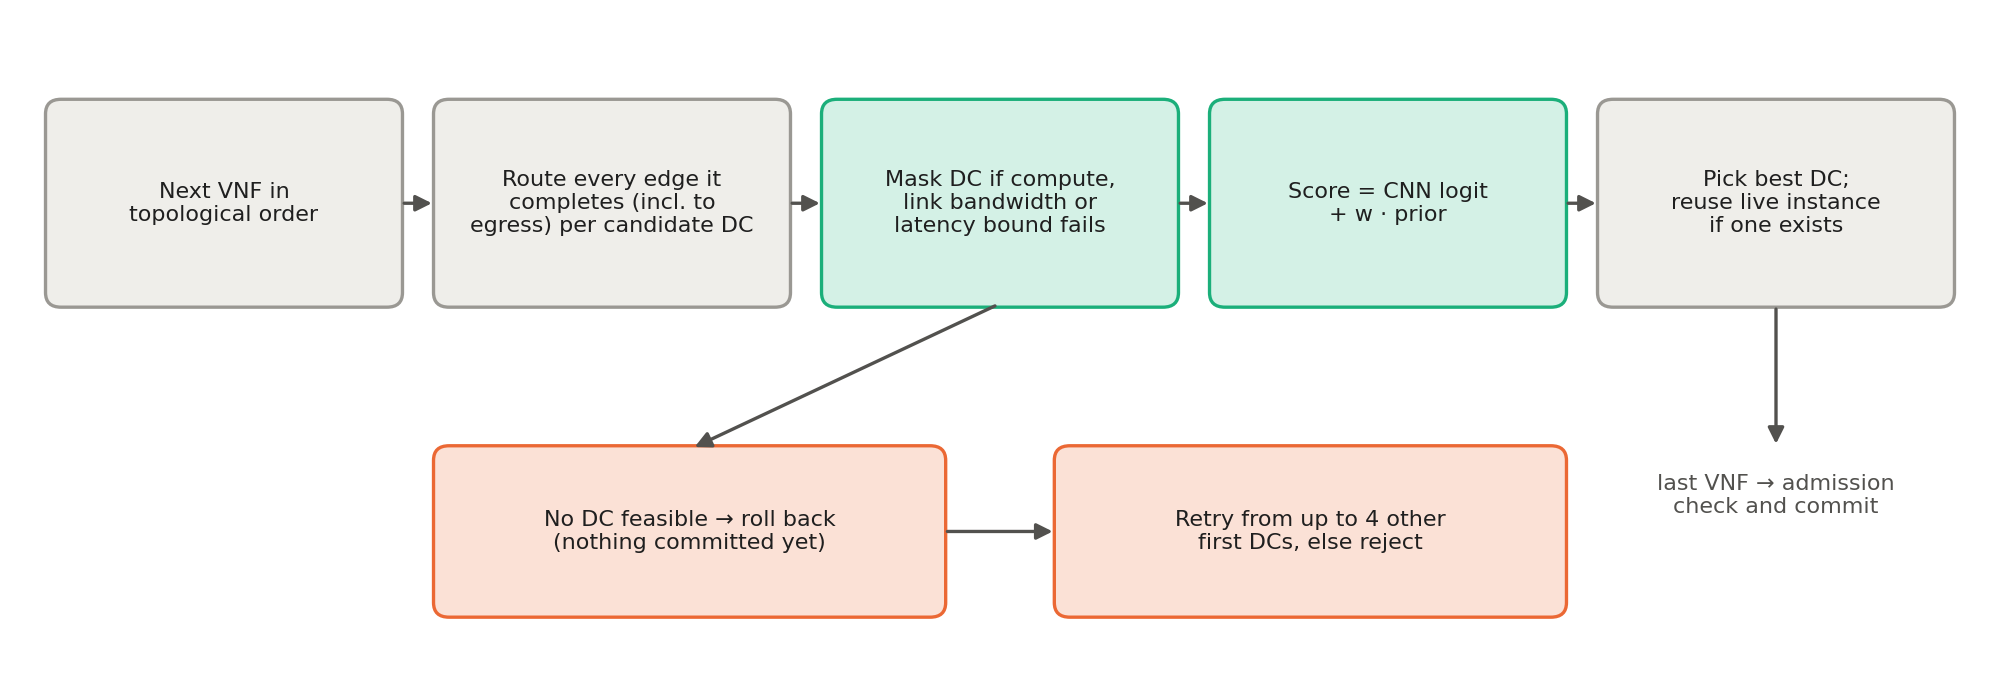
\includegraphics[width=0.95\linewidth]{placement-flow.png}
\caption{One placement decision in the updated FPPVS.}
\label{fig:flow}
\end{figure}

\begin{algorithm}[H]
\caption{Updated FPPVS admission for one request $u$}\label{alg:place}
\begin{algorithmic}[1]
\Require request $u$, ledger $\mathcal{L}$, policy $\pi_\theta$, retries $K$
\State $G_u \gets$ \Call{Parallelize}{$u$} \Comment{Algorithm 1 of the paper}
\For{attempt $= 0,\dots,K$}
  \State reset episode state (nothing is committed yet)
  \For{each VNF $f$ of $u$ in order}
    \For{each DC $v$}
      \State route the edges of $G_u$ completed by putting $f$ on $v$
      \State $m_v \gets$ compute, bandwidth and latency bound all hold
    \EndFor
    \If{no $m_v$ is true} \State \textbf{break} \Comment{dead end, try next attempt} \EndIf
    \If{$f$ is the first VNF and attempt $>0$}
      \State $v^\ast \gets$ the attempt-th best DC by prior score, excluding the policy's choice
    \Else
      \State $v^\ast \gets \arg\max_{v:\,m_v} \big(\text{logit}_\theta(s)_v + w\cdot \text{prior}_v\big)$
    \EndIf
    \State place $f$ on $v^\ast$; reuse a live instance of its type on $v^\ast$ if sharing is on
  \EndFor
  \If{all VNFs placed \textbf{and} \Call{Evaluate}{$G_u$} feasible \textbf{and} fits $\mathcal{L}$}
    \State commit to $\mathcal{L}$ until $t_u+\tau_u$; \Return accept
  \EndIf
\EndFor
\State \Return reject
\end{algorithmic}
\end{algorithm}

\subsection{MDP: state, action and mask}
\textbf{State.} A $9\times|V_s|$ grid, one column per DC (Table~\ref{tab:state}).

\begin{table}[H]
\centering\small
\caption{State features per DC column. Rows marked ``ours'' were added by us.}
\label{tab:state}
\begin{tabular}{clc}
\toprule
Row & Feature & Origin \\
\midrule
1 & Residual compute fraction (includes all active SFCs) & paper, fixed by us \\
2 & Demand of the current VNF / capacity & paper \\
3 & Latency from the DC of the previous VNF & paper \\
4 & Latency to the destination & \ours{ours} \\
5 & Smallest remaining bandwidth fraction on newly routed links & \ours{ours} \\
6 & A live instance of this VNF type exists (reuse possible) & \ours{ours} \\
7 & SQN-LSTM demand forecast for this VNF type & paper \\
8 & Placement prior score & \ours{ours} \\
9 & Feasibility mask & \ours{ours} \\
\bottomrule
\end{tabular}
\end{table}

\textbf{Action.} Choose one DC for the current VNF. \textbf{Mask.} A DC is
allowed only if (i) its residual compute covers the VNF demand plus instance
overhead when a new instance is needed, (ii) every link on the newly routed
paths still has the data rate free, and (iii) the critical-path latency so far
plus the shortest latency from the DC to the destination is within $L^{\max}_u$.
Because shortest-path latency obeys the triangle inequality, (iii) never removes
a DC that could still lead to a valid placement.

\subsection{Placement prior}
The prior score of DC $v$ for VNF $f$ is
\begin{equation}
\begin{split}
\text{prior}_v ={}& -(h^{new}_v + h^{dst}_v) - 2\,\frac{T_v + L(v,d_u)}{L^{\max}_u}
 + 0.5\,\mathbf{1}[\text{reuse}] \\
 & + 0.3\,\mathbf{1}[v = v_{prev}] + 0.5\,\tilde{C}_v - 3\,\frac{\max(0,\,0.25-\beta_v)}{0.25},
\end{split}
\end{equation}
where $h^{new}_v$ is the number of link hops (weighted by data rate) the new
edges use, $h^{dst}_v$ the hops from $v$ to the destination, $T_v$ the
critical-path finish time of $f$ on $v$, $\tilde C_v$ the residual compute
fraction after placement and $\beta_v$ the bandwidth margin. In words: keep the
chain short and on few DCs, reuse live instances, avoid nearly full DCs and
links.

\subsection{Actor-critic network}
The paper's three convolutional layers with 64 filters, batch normalization and
ReLU are kept, but the kernels are $3\times1$, running along the feature axis
only, because neighbouring columns are unrelated DCs. The \textbf{actor} applies
the same two $1\times1$ convolutions to every column, averages over the feature
axis and outputs one logit per DC; we add $w\cdot\text{prior}$, where $w$ is a
learnable scalar (initial value 2). The network therefore learns a correction on
top of a sensible rule, and it is permutation-equivariant: reordering the DCs
reorders the outputs in the same way (this is checked by a unit test). The
\textbf{critic} keeps the paper's design: global pooling, a 256-unit fully
connected layer, dropout 0.3 and one output.

\subsection{Reward}\label{sec:reward}
Following Eq.~(28) of the paper: $+1$ for each valid placement, $-1$ when a new
instance must be started, and $-10$ if the request is rejected. We added a small
bandwidth term ($-0.2$ per data-rate-weighted hop) and dropped the paper's $+5$
reuse bonus, because the prior already rewards reuse. When the request is
accepted, the agent gets $5\,(1 + \max(0,1 - L_u/L^{\max}_u))$, which rewards
latency slack, plus a fairness bonus $5\,\Delta\mathrm{JFI}$ (the change in
Jain's index~\cite{jain} over the throughputs of accepted requests).

\subsection{Training}
Each episode is trained with advantage actor-critic~\cite{a3c}: discounted
returns, advantage = return $-$ critic value, actor loss with an entropy bonus,
critic MSE loss, and gradient clipping. Exploration combines the paper's
adaptive $\epsilon$-greedy rule ($\epsilon$ shrinks after an accepted request
and grows after a rejection) with small Gaussian noise on the logits. Four
agents train locally for 50 episodes per round on their own request streams and
ledgers, continuing through the stream from round to round; the server then
averages their weights, weighted by the number of episodes. Evaluation is
deterministic (arg-max over allowed DCs) on a hold-out stream that is never used
for training. Table~\ref{tab:hyper} lists the hyperparameters.

\begin{table}[H]
\centering\small
\caption{Training hyperparameters.}
\label{tab:hyper}
\begin{tabular}{ll@{\qquad}ll}
\toprule
Optimizer & Adam, lr $5\times10^{-4}$ & Discount $\gamma$ & 0.99 \\
Federated agents & 4 & FedAvg rounds & 10 \\
Episodes per agent per round & 50 & Total training episodes & 2000 \\
$\epsilon$ start / min / decay & 0.15 / 0.02 / 0.995 & Logit noise std & 0.10 \\
Entropy coefficient & 0.01 & Gradient clip & 1.0 \\
Critic loss weight & 0.5 & Prior weight $w$ (initial) & 2.0 (learned) \\
SQN depth / LSTM hidden & 5 / 64 & Retries $K$ & 4 \\
Instance overhead $o$ & 0.25 units & Training requests per agent & 600 \\
\bottomrule
\end{tabular}
\end{table}

%=====================================================================
\section{Performance Evaluation}
%=====================================================================

\subsection{Experimental setup}
\textbf{Hardware:} laptop with a 12th Gen Intel Core i5-12500H CPU and 16 GB of
RAM, running Windows 11. No GPU was used. \textbf{Software:} Python 3.12.1,
PyTorch 2.10 (CPU build), NetworkX 3.6.1 and Matplotlib 3.10.8. Scenarios run in
parallel worker processes with one PyTorch thread each. Each scenario is
repeated with \numSeeds{} seeds (7--11). For each seed we generate a new network,
four training streams and one hold-out stream. Training one FPPVS model takes
about \trainSeconds\,s.

\begin{table}[H]
\centering\small
\caption{Simulation parameters. Values follow Section 5.1 of the paper unless
marked as ours.}
\label{tab:params}
\begin{tabularx}{\linewidth}{l X}
\toprule
Parameter & Value \\
\midrule
Topologies & Backbone: 24 DCs, 47 links; Metro: 17 DCs, 29 links (random connected graphs) \\
DC compute capacity & $\mathcal{U}(10, 20)$ units \\
Link bandwidth & 100--200 units in steps of 20 \\
Link latency & $\mathcal{U}(5, 20)$ ms \\
SFC length & 4--10 VNFs, types IDS, DPI, LB, FW, NAT \\
Monitor probability (IDS/DPI) & 0.45; a monitor gates a later shaper with prob.\ 0.5 \\
VNF compute demand & $\mathcal{U}(0.5, 0.9)$ units (500--900 Mbps normalized) \\
VNF processing latency & $\mathcal{U}(0.01, 0.2)$ ms \\
Data rate per request & bounded power law on $[5, 30]$, exponent 1.5 \\
Maximum latency & $\mathcal{U}(100, 150)$ ms \\
Lifetime (TTL) & exponential, mean 1000 time units \\
Arrivals & \ours{Poisson, rate set by offered load $\rho$} \\
Offered load $\rho$ & \ours{0.5, 0.75, 1.0 (main); 1.25, 1.5 (stress)} \\
Instance overhead & \ours{0.25 units per live instance} \\
Requests per stream & \ours{600 hold-out; 600 per training agent} \\
\bottomrule
\end{tabularx}
\end{table}

\subsection{Performance metrics}
\begin{itemize}
  \item \textbf{Service acceptance}: accepted hold-out requests divided by all
  hold-out requests (higher is better).
  \item \textbf{Compute / bandwidth per running SFC}: time-averaged compute (or
  bandwidth) in use divided by the time-averaged number of running SFCs. This is
  the amount of resources one service holds at any moment (lower is better).
  \item \textbf{Compute$\cdot$time and bandwidth$\cdot$time per accepted SFC}:
  $R_{comp}$ and $R_{bw}$ from Section 4 (lower is better).
  \item \textbf{Instances per accepted SFC}: VNF instances started divided by
  accepted requests; this measures how much sharing is used (lower is better).
  \item \textbf{Latency}: mean critical-path end-to-end latency of accepted
  requests.
  \item \textbf{Decision time}: wall-clock time per request, including retries.
\end{itemize}

\subsection{Compared methods}
We compare five methods. All of them run in the same simulator, on the same
networks, training streams and hold-out requests, with the same instance model
(M2), so none of them can overbook capacity. The three learning methods get the
same training budget of 2000 episodes.
\begin{itemize}
  \item \textbf{Updated FPPVS (ours):} the method of Section~\ref{sec:approach}.
  \item \textbf{Original FPPVS} (Zhu et al.~\cite{fppvs}), run as the paper
  describes it: the paper's four-row state (residual capacity, VNF demand,
  distance from the previous VNF, SQN-LSTM forecast), pruning by compute only,
  the paper's CNN (three $3\times3$ convolution layers with 64 filters, global
  pooling, a 256-unit layer with dropout 0.3, one output per DC), the paper's
  step reward (Eq.~28: $+1$ valid, $+5$ reuse, $-1$ new instance, $-10$
  rejection), adaptive $\epsilon$-greedy exploration and federated training
  (4 agents, 10 rounds, 50 episodes). No look-ahead mask, no prior and no
  retries.
  \item \textbf{2022 adaptation} of Zhang et al.~\cite{zhang2022}: online SFC
  placement with sequential VNF placement (no parallelization), reuse of an
  existing same-type VNF, an SQN-LSTM queue of depth $T_D=20$ for demand
  forecasting, an actor-critic placement policy (a fully connected network over
  the same four-row state), and rollback when a request cannot be completed.
  Its reward follows the long-term revenue-to-cost ratio (LTCR): on success the
  agent receives $10\cdot\min(2,\ \text{revenue}/\text{cost})$, where revenue is
  the requested compute plus bandwidth and cost is the compute and link
  bandwidth actually used; a failure gets a fixed penalty of $-10$. It is
  trained by a single synchronous agent. This is our adaptation from the
  method description; the authors' code was not available.
  \item \textbf{Greedy:} the feasible DC with the most residual compute (load
  balancing), without sharing.
  \item \textbf{Random:} a random feasible DC, without sharing.
\end{itemize}
Greedy and random use our feasibility mask, so they never pick a DC that is
already known to be infeasible. We also compare against the numbers published in
the FPPVS paper (Section~\ref{sec:paper}). Separately, an ablation study switches
off one part of updated FPPVS at a time (no sharing, no fairness bonus, a single
agent, no retries, and the placement prior alone without learning).

\subsection{Results}

% Results section, included from report.tex. All tables are generated by
% scripts/make_report_tables.py from output/scenarios/scenario-results.json.

\subsubsection*{A. Service acceptance}

Table~\ref{tab:acc} and Figure~\ref{fig:acc} give hold-out acceptance for every
scenario. Updated FPPVS reaches the 70\% target in all six main scenarios. Its
mean acceptance ranges from \fppvsMinAcc\% (\fppvsWorstScenario) to
\fppvsMaxAcc\%, with an average of \fppvsMeanAcc\%. The lowest value in any single
seed was \fppvsLowestRun\%, so the target also holds run by run, not only on
average.

\begin{table}[H]
\centering\footnotesize
\setlength{\tabcolsep}{4pt}
\caption{Hold-out service acceptance (\%), mean $\pm$ standard deviation over
\numSeeds{} seeds. Best value per row in bold.}
\label{tab:acc}
\begin{tabular}{lccccc}
\toprule
Scenario (topology, load) & Updated (ours) & Original FPPVS & 2022 adaptation & Greedy & Random \\
\midrule
Backbone 0.5 & \textbf{99.6 $\pm$ 0.4} & 58.1 $\pm$ 4.1 & 68.1 $\pm$ 5.4 & 72.1 $\pm$ 5.8 & 73.2 $\pm$ 4.5 \\
Backbone 0.75 & \textbf{97.2 $\pm$ 2.1} & 50.1 $\pm$ 3.7 & 48.6 $\pm$ 15.3 & 62.6 $\pm$ 5.7 & 61.8 $\pm$ 3.8 \\
Backbone 1 & \textbf{86.4 $\pm$ 3.7} & 43.6 $\pm$ 5.1 & 44.5 $\pm$ 6.5 & 53.4 $\pm$ 5.1 & 55.3 $\pm$ 3.4 \\
Metro 0.5 & \textbf{99.0 $\pm$ 0.8} & 64.6 $\pm$ 10.2 & 74.0 $\pm$ 9.7 & 71.4 $\pm$ 3.0 & 72.1 $\pm$ 2.9 \\
Metro 0.75 & \textbf{93.0 $\pm$ 2.5} & 58.5 $\pm$ 6.6 & 59.1 $\pm$ 5.3 & 59.5 $\pm$ 2.9 & 59.9 $\pm$ 2.3 \\
Metro 1 & \textbf{81.3 $\pm$ 3.5} & 49.7 $\pm$ 4.5 & 49.4 $\pm$ 9.7 & 51.8 $\pm$ 3.6 & 52.6 $\pm$ 3.0 \\
\midrule \multicolumn{6}{l}{\emph{Overload stress tests (offered demand above total capacity)}} \\
Backbone 1.25 & \textbf{75.2 $\pm$ 2.9} & 38.7 $\pm$ 3.9 & 41.1 $\pm$ 3.0 & 49.3 $\pm$ 3.8 & 50.9 $\pm$ 2.7 \\
Backbone 1.5 & \textbf{65.2 $\pm$ 3.3} & 35.0 $\pm$ 4.2 & 38.4 $\pm$ 4.3 & 43.4 $\pm$ 4.1 & 44.2 $\pm$ 2.1 \\
Metro 1.25 & \textbf{69.2 $\pm$ 4.2} & 44.0 $\pm$ 2.9 & 40.5 $\pm$ 7.8 & 47.2 $\pm$ 2.1 & 46.9 $\pm$ 2.3 \\
Metro 1.5 & \textbf{60.6 $\pm$ 1.9} & 36.7 $\pm$ 5.0 & 42.2 $\pm$ 3.9 & 42.2 $\pm$ 2.7 & 43.1 $\pm$ 1.3 \\
\bottomrule
\end{tabular}
\end{table}

\begin{figure}[H]
\centering
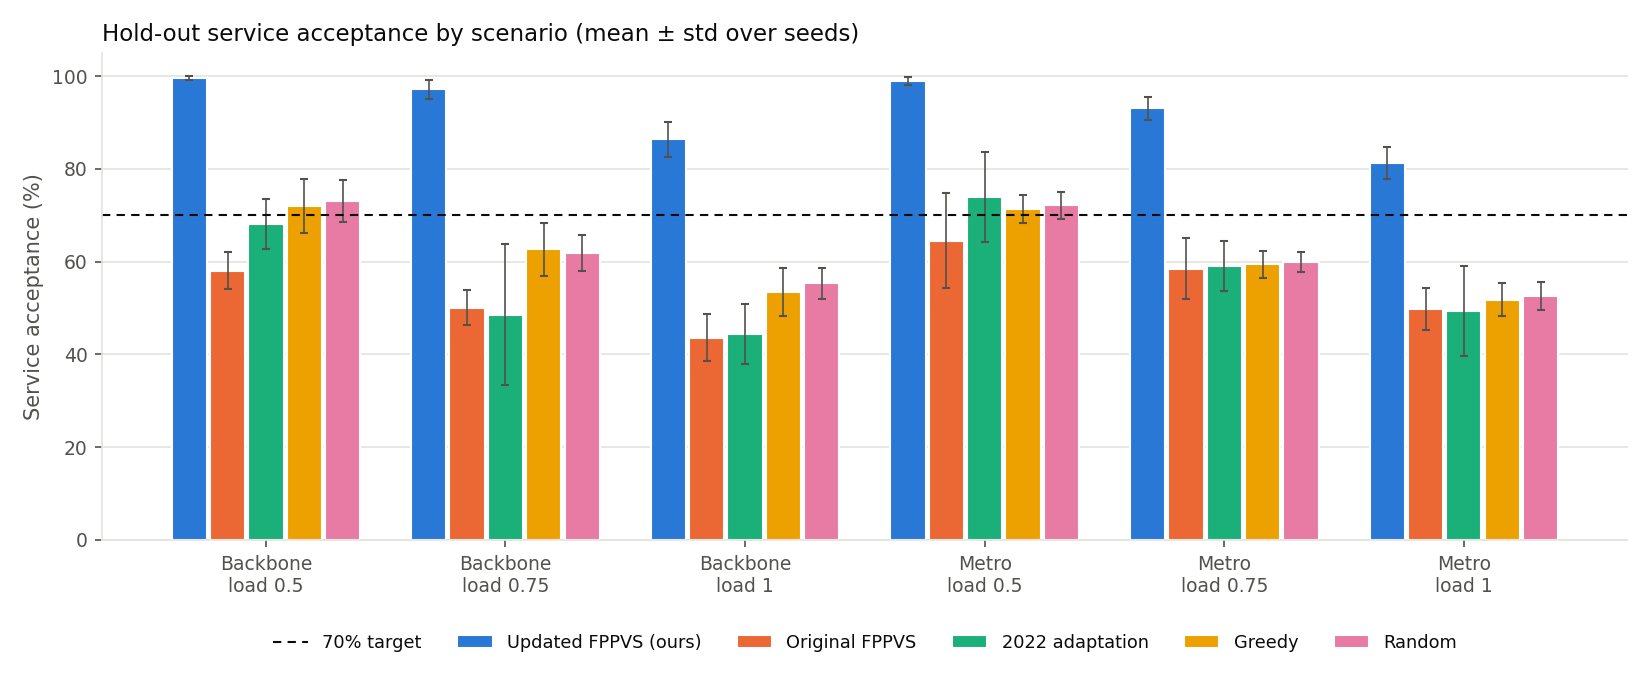
\includegraphics[width=\linewidth]{scenario-acceptance.png}
\caption{Hold-out acceptance per scenario. Error bars show one standard
deviation over seeds; the dashed line is the 70\% target.}
\label{fig:acc}
\end{figure}

\needspace{5\baselineskip}
\paragraph{Observations.}
\begin{itemize}
  \item Updated FPPVS is the best method in every scenario. At full load
  ($\rho=1$) it accepts 86.4\% on Backbone and 81.3\% on Metro.
  \item The original FPPVS reaches \origMinAcc--\origMaxAcc\% in the main
  scenarios (mean \origMeanAcc\%), and the 2022 adaptation reaches
  \zhangMinAcc--\zhangMaxAcc\% (mean \zhangMeanAcc\%). Updated FPPVS is
  \origGainMean{} points above the original and \zhangGainMean{} points above
  the 2022 adaptation on average.
  \item Both learning baselines often score below greedy and random. The
  reason is how infeasible choices are handled. Greedy and random run with our
  feasibility mask, so they never pick a DC that is already known to break
  bandwidth or latency. The original FPPVS and the 2022 adaptation check only
  compute while placing, as their methods describe, and find bandwidth and
  latency violations only when the whole chain is done (see Part E).
  \item The 2022 adaptation is the least stable method: its standard deviation
  across seeds reaches 15 points (Backbone, $\rho=0.75$). One reward value per
  episode (LTCR) gives the agent a weak learning signal.
  \item Greedy and random accept only 52--73\% even at light load. They spread
  VNFs over many DCs, so each request uses two to three times as much link
  bandwidth as updated FPPVS (Section~C), and links run out first.
  \item Metro is harder than Backbone at the same load. It has fewer DCs and
  fewer links, so there are fewer alternative paths when a link fills up.
\end{itemize}

\begin{figure}[H]
\centering
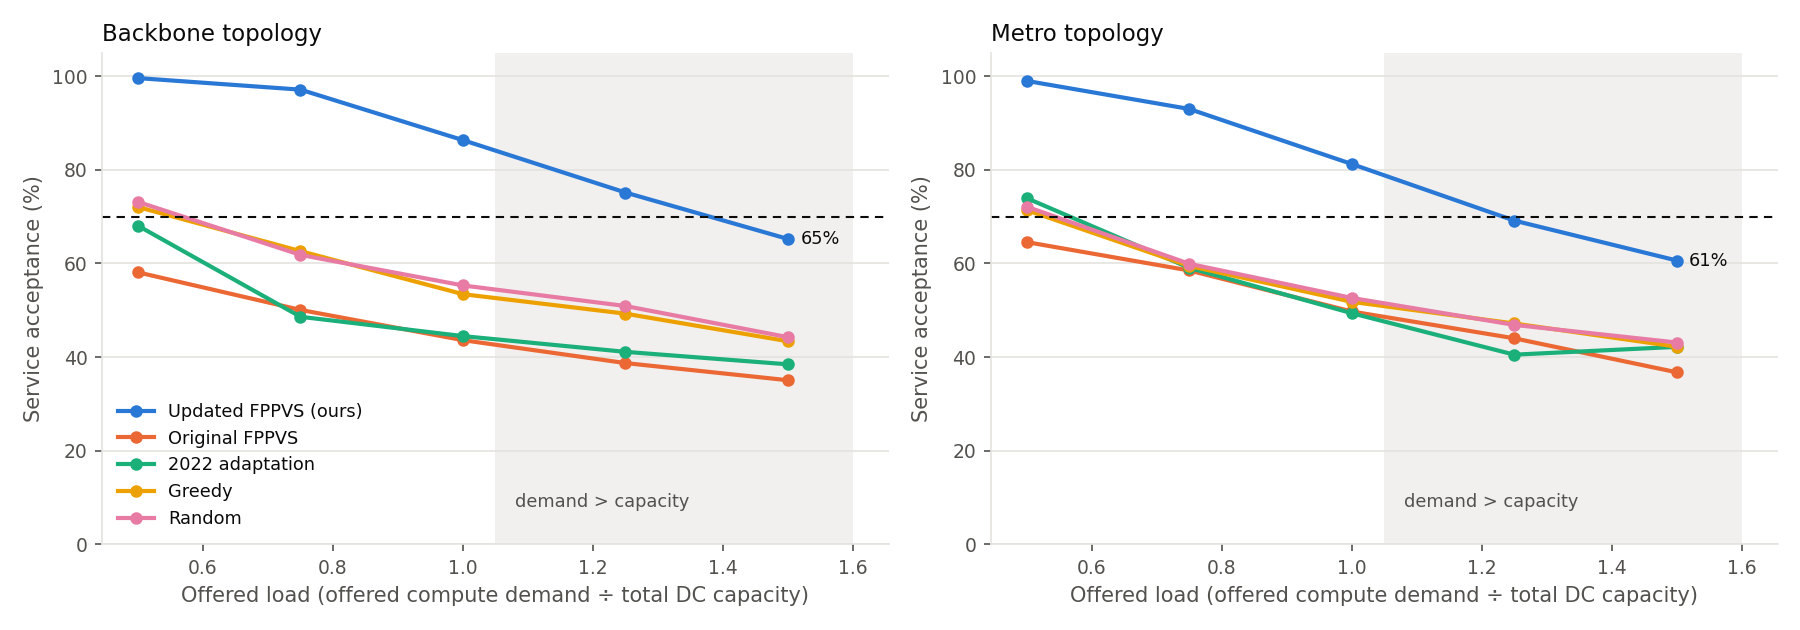
\includegraphics[width=\linewidth]{load-sweep.png}
\caption{Acceptance against offered load. The shaded area is overload, where the
average offered compute is larger than the total compute of the network.}
\label{fig:sweep}
\end{figure}

\paragraph{Overload.} Figure~\ref{fig:sweep} extends the load to 1.5 times the
network capacity. Updated FPPVS stays clearly ahead at every point: 75.2\%
(Backbone) and 69.2\% (Metro) at $\rho=1.25$, and 65.2\% and 60.6\% at
$\rho=1.5$. All other methods stay at or below 51\%. Below 70\% is unavoidable in
this region. At $\rho=1.5$ only about two thirds of the offered compute can fit
in the network at any time, whatever the placement policy. We therefore treat
these points as stress tests and not as part of the 70\% target.

\subsubsection*{B. Ablation study}

\begin{table}[H]
\centering\small
\caption{Ablation: hold-out acceptance (\%) of updated FPPVS with one part
switched off at a time.}
\label{tab:ablation}
\begin{tabular}{lcccccc}
\toprule
Scenario & Full & w/o sharing & w/o fairness & 1 agent & w/o retry & Prior only \\
\midrule
Backbone 0.5 & 99.6 $\pm$ 0.4 & 99.0 $\pm$ 1.0 & 99.4 $\pm$ 0.6 & 99.4 $\pm$ 0.6 & 99.5 $\pm$ 0.4 & 99.7 $\pm$ 0.3 \\
Backbone 0.75 & 97.2 $\pm$ 2.1 & 87.5 $\pm$ 3.0 & 97.0 $\pm$ 1.8 & 96.5 $\pm$ 2.2 & 96.7 $\pm$ 2.4 & 96.9 $\pm$ 2.2 \\
Backbone 1 & 86.4 $\pm$ 3.7 & 73.8 $\pm$ 3.1 & 85.6 $\pm$ 3.9 & 86.0 $\pm$ 3.4 & 85.4 $\pm$ 3.1 & 86.3 $\pm$ 2.8 \\
Metro 0.5 & 99.0 $\pm$ 0.8 & 97.9 $\pm$ 1.1 & 99.1 $\pm$ 1.0 & 98.5 $\pm$ 1.3 & 98.8 $\pm$ 0.9 & 99.0 $\pm$ 0.6 \\
Metro 0.75 & 93.0 $\pm$ 2.5 & 84.1 $\pm$ 2.3 & 93.4 $\pm$ 2.8 & 93.5 $\pm$ 3.2 & 93.5 $\pm$ 2.9 & 94.1 $\pm$ 2.2 \\
Metro 1 & 81.3 $\pm$ 3.5 & 70.6 $\pm$ 3.2 & 81.1 $\pm$ 2.9 & 81.0 $\pm$ 3.2 & 81.9 $\pm$ 4.0 & 81.7 $\pm$ 3.2 \\
\bottomrule
\end{tabular}
\end{table}

Table~\ref{tab:ablation} switches off one part of updated FPPVS at a time.
\begin{itemize}
  \item \textbf{VNF sharing matters most.} Without it, acceptance falls by 9--13
  points at $\rho\ge0.75$ (for example 86.4\% to 73.8\% on Backbone at
  $\rho=1$). Every VNF then pays its own instance overhead, so the DCs fill up
  sooner.
  \item \textbf{Fairness bonus, single vs.\ federated training and retries}
  change acceptance by about one point or less, which is within the
  seed-to-seed spread. Fairness is meant to balance throughput between flows, not
  to raise acceptance, so this is expected. Retries help only in the rare case
  where the first placement hits a dead end.
  \item \textbf{The learned network adds little over its prior.} ``Prior only''
  uses the same mask, prior and retries with no neural network, and it is within
  about one point of the full method everywhere. We report this openly: in our
  experiments the gains come mainly from the problem modifications (mask, sharing
  model, prior), not from the reinforcement learning itself. One reason is
  limitation L6: each episode covers only one request, so the agent sees little
  of the long-term effect of its choices.
\end{itemize}

\subsubsection*{C. Resource usage}

Figure~\ref{fig:res} and Table~\ref{tab:res} show the resources each method holds
for the services it runs. Table~\ref{tab:savings} summarises the difference
between updated FPPVS and each other method, averaged over the six main
scenarios.

\begin{figure}[H]
\centering
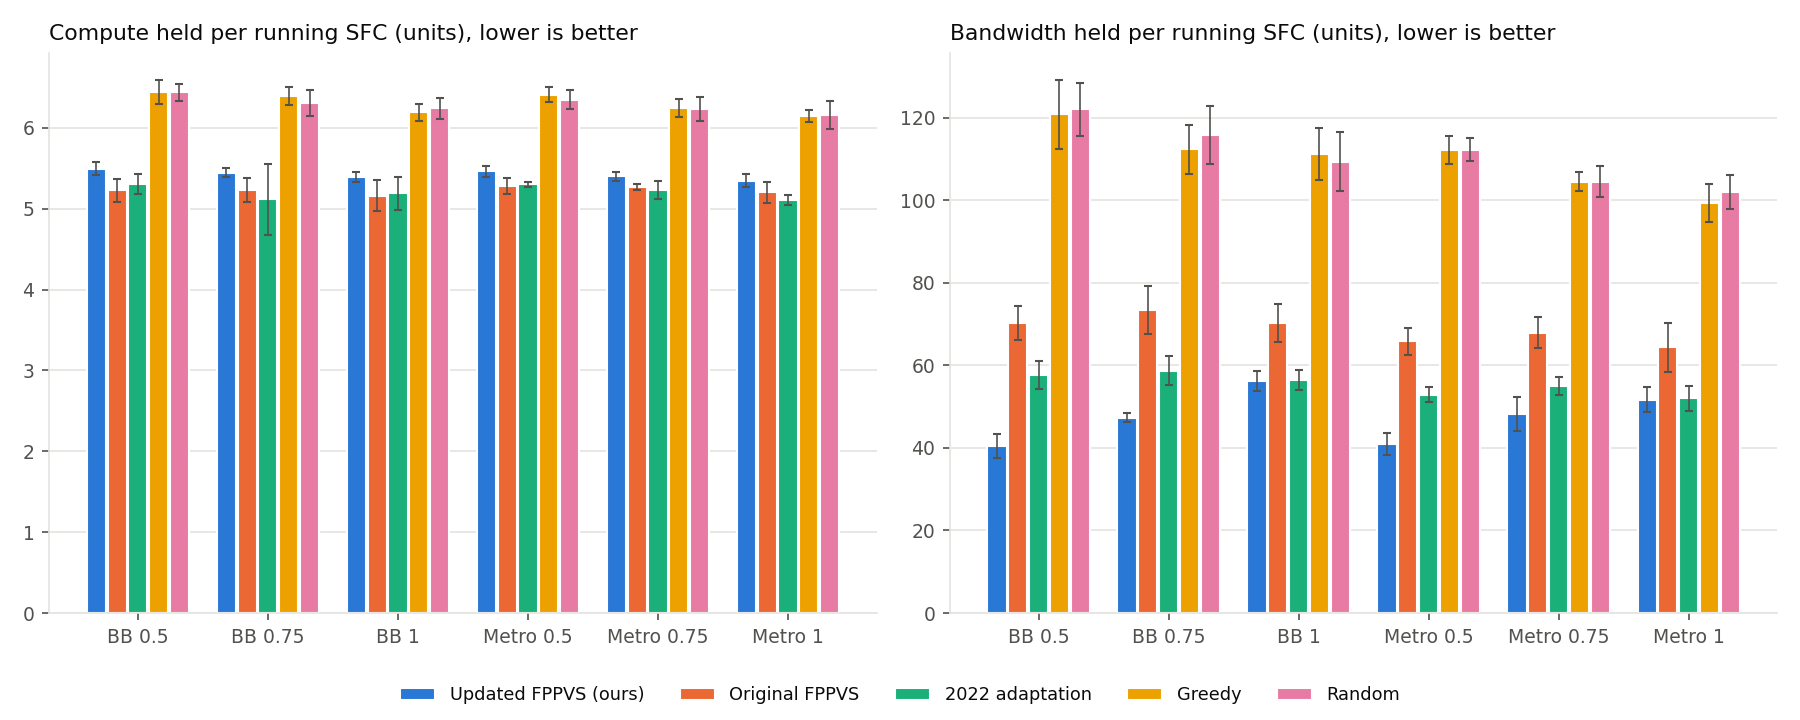
\includegraphics[width=\linewidth]{scenario-resources.png}
\caption{Compute (left) and bandwidth (right) held per running SFC, averaged over
time. Lower means each service costs less to keep running.}
\label{fig:res}
\end{figure}

\begin{table}[H]
\centering\small
\caption{Average reduction in resource use achieved by updated FPPVS over each
method (main scenarios; positive means updated FPPVS uses less, negative means
it uses more).}
\label{tab:savings}
\begin{tabular}{lcccc}
\toprule
Reduction vs. & Compute & Bandwidth & BW$\cdot$time & Instances \\
 & per SFC & per SFC & per accepted & per accepted \\
\midrule
Original FPPVS & -3.7\% & +30.7\% & +30.8\% & -6.5\% \\
2022 adaptation & -4.1\% & +14.2\% & +15.0\% & -8.3\% \\
Greedy & +14.0\% & +56.5\% & +57.1\% & +89.8\% \\
Random & +13.7\% & +56.9\% & +57.4\% & +89.8\% \\
\bottomrule
\end{tabular}
\end{table}

\begin{table}[H]
\centering\scriptsize
\setlength{\tabcolsep}{4pt}
\caption{Resource use and latency per scenario (mean over seeds; best per
column within a scenario in bold). ``Per acc.'' means per accepted SFC.}
\label{tab:res}
\begin{tabular}{llcccccc}
\toprule
Scenario & Method & Compute & Bandwidth & Compute$\cdot$time & BW$\cdot$time & Instances & Latency \\
 & & per SFC & per SFC & per acc. ($10^3$) & per acc. ($10^3$) & per acc. & (ms) \\
\midrule
Backbone 0.5 & Updated (ours) & 5.49 & \textbf{40.5} & 5.49 & \textbf{40.5} & 0.86 & \textbf{33.3} \\
 & Original FPPVS & \textbf{5.23} & 70.2 & \textbf{5.26} & 70.6 & 0.63 & 62.7 \\
 & 2022 adaptation & 5.31 & 57.6 & 5.35 & 58.0 & \textbf{0.60} & 64.7 \\
 & Greedy & 6.45 & 120.8 & 6.46 & 120.9 & 6.82 & 111.0 \\
 & Random & 6.44 & 122.0 & 6.53 & 123.7 & 6.77 & 111.6 \\
\midrule
Backbone 0.75 & Updated (ours) & 5.45 & \textbf{47.4} & 5.43 & \textbf{47.2} & 0.65 & \textbf{38.9} \\
 & Original FPPVS & 5.23 & 73.4 & 5.30 & 74.5 & \textbf{0.58} & 63.0 \\
 & 2022 adaptation & \textbf{5.11} & 58.7 & \textbf{5.19} & 59.8 & 0.62 & 68.1 \\
 & Greedy & 6.40 & 112.3 & 6.50 & 114.1 & 6.75 & 109.0 \\
 & Random & 6.31 & 115.9 & 6.38 & 117.3 & 6.64 & 109.8 \\
\midrule
Backbone 1 & Updated (ours) & 5.39 & \textbf{56.2} & 5.42 & \textbf{56.5} & \textbf{0.53} & \textbf{50.0} \\
 & Original FPPVS & \textbf{5.16} & 70.2 & \textbf{5.20} & 70.8 & 0.59 & 64.2 \\
 & 2022 adaptation & 5.19 & 56.5 & 5.28 & 57.4 & 0.61 & 67.2 \\
 & Greedy & 6.19 & 111.2 & 6.40 & 115.1 & 6.58 & 107.7 \\
 & Random & 6.24 & 109.4 & 6.27 & 110.1 & 6.58 & 108.1 \\
\midrule
Metro 0.5 & Updated (ours) & 5.46 & \textbf{41.0} & 5.57 & \textbf{41.9} & 0.85 & \textbf{33.7} \\
 & Original FPPVS & \textbf{5.28} & 65.8 & \textbf{5.31} & 66.3 & 0.70 & 56.7 \\
 & 2022 adaptation & 5.30 & 52.9 & 5.40 & 53.8 & \textbf{0.69} & 64.2 \\
 & Greedy & 6.41 & 112.2 & 6.44 & 112.7 & 6.76 & 109.2 \\
 & Random & 6.35 & 112.3 & 6.50 & 115.1 & 6.67 & 109.3 \\
\midrule
Metro 0.75 & Updated (ours) & 5.40 & \textbf{48.2} & 5.52 & \textbf{49.4} & 0.65 & \textbf{40.8} \\
 & Original FPPVS & 5.27 & 67.9 & 5.39 & 69.5 & 0.65 & 62.5 \\
 & 2022 adaptation & \textbf{5.23} & 55.0 & \textbf{5.32} & 55.9 & \textbf{0.63} & 67.4 \\
 & Greedy & 6.25 & 104.5 & 6.43 & 107.6 & 6.63 & 105.8 \\
 & Random & 6.23 & 104.5 & 6.52 & 109.5 & 6.61 & 107.2 \\
\midrule
Metro 1 & Updated (ours) & 5.35 & \textbf{51.6} & 5.44 & \textbf{52.5} & \textbf{0.55} & \textbf{48.6} \\
 & Original FPPVS & 5.21 & 64.3 & \textbf{5.28} & 65.4 & 0.67 & 62.2 \\
 & 2022 adaptation & \textbf{5.11} & 52.0 & 5.35 & 54.4 & 0.62 & 67.2 \\
 & Greedy & 6.15 & 99.4 & 6.46 & 104.4 & 6.53 & 104.1 \\
 & Random & 6.16 & 101.9 & 6.38 & 105.6 & 6.51 & 105.2 \\
\bottomrule
\end{tabular}
\end{table}

\needspace{5\baselineskip}
\paragraph{Observations.}
\begin{itemize}
  \item \textbf{Bandwidth.} Updated FPPVS holds the least bandwidth per running
  SFC in every main scenario: about 57\% less than greedy and random, 31\% less
  than the original FPPVS and 14\% less than the 2022 adaptation. Most of the
  saving comes from keeping consecutive VNFs on the same DC.
  \item \textbf{Compute and instances.} Against greedy and random, which do not
  share VNFs, updated FPPVS needs about 14\% less compute per service and about
  90\% fewer new instances (0.5--0.9 per accepted SFC instead of about 7).
  Against the original FPPVS and the 2022 adaptation, which both share VNFs, it
  uses about 4\% more compute per service and 7--8\% more instances per accepted
  request. Those two methods accept only about half of the requests, most likely
  the ones that were easy to fit, so their per-request averages come from an
  easier set. Even so, the difference is small next to the 35--39 points of
  extra acceptance.
  \item \textbf{Latency.} Mean latency of accepted requests is 33--50\,ms for
  updated FPPVS, 57--68\,ms for the original FPPVS and the 2022 adaptation,
  and 104--111\,ms for greedy and random. All are below the 100--150\,ms limits.
  The 2022 adaptation places the chain strictly in sequence (no parallel
  branches), so every monitor adds to the critical path.
  \item \textbf{Decision time.} Updated FPPVS needs 9--21\,ms per request,
  including the CNN forward pass and occasional retries. Greedy and random take
  about 3\,ms. Training one updated FPPVS model with 2000 episodes takes about
  \trainSeconds\,s on the CPU.
\end{itemize}

\subsubsection*{D. Effect of the algorithm alone}

Our main experiments use a different arrival process from our first version
(modification M1). To separate the effect of the algorithm from the effect of the
workload, we also ran the updated placement logic on the original workload: one
arrival per time unit, 100 requests, with almost nothing released during the run
(Table~\ref{tab:old}). The updated placement reaches 70.4\%, up from 10.4\% for
the original implementation. Acceptance is lower than in the Poisson runs mainly
because the original stream offers far more traffic than the network can hold.

\begin{table}[H]
\centering\small
\caption{Original workload (one arrival per time unit), 5 seeds. The upper
rows are from our first implementation; the lower rows use the updated
environment and placement logic.}
\label{tab:old}
\begin{tabular}{lc}
\toprule
Method (original workload, 100 requests) & Acceptance (\%) \\
\midrule
Original implementation, trained FDRL (5 seeds) & 10.4 $\pm$ 5.1 \\
Original implementation, greedy & 15.8 $\pm$ 3.1 \\
Original implementation, random & 11.6 $\pm$ 3.0 \\
\midrule
Updated FPPVS placement & 70.4 $\pm$ 2.9 \\
Greedy & 45.4 $\pm$ 2.1 \\
Random & 46.2 $\pm$ 2.2 \\
\bottomrule
\end{tabular}
\end{table}

\subsubsection*{E. Comparison with the original FPPVS and the 2022 adaptation}\label{sec:paper}

\paragraph{Same scenarios, same requests.} Table~\ref{tab:orig} puts the three
learning-based methods side by side. All three get 2000 training episodes and
are tested on the same hold-out requests.

\begin{table}[H]
\centering\small
\caption{Original FPPVS, the 2022 adaptation and updated FPPVS on identical
scenarios, mean over \numSeeds{} seeds. $^\ast$Gain = updated FPPVS minus the
better of the other two, in percentage points.}
\label{tab:orig}
\begin{tabular}{lccccccc}
\toprule
 & \multicolumn{4}{c}{Acceptance (\%)} & \multicolumn{3}{c}{Bandwidth per running SFC} \\
\cmidrule(lr){2-5}\cmidrule(lr){6-8}
Scenario & Original & 2022 & Updated & Gain$^\ast$ & Original & 2022 & Updated \\
\midrule
Backbone 0.5 & 58.1 & 68.1 & \textbf{99.6} & +31.6 & 70.2 & 57.6 & \textbf{40.5} \\
Backbone 0.75 & 50.1 & 48.6 & \textbf{97.2} & +47.1 & 73.4 & 58.7 & \textbf{47.4} \\
Backbone 1 & 43.6 & 44.5 & \textbf{86.4} & +41.9 & 70.2 & 56.5 & \textbf{56.2} \\
Metro 0.5 & 64.6 & 74.0 & \textbf{99.0} & +25.1 & 65.8 & 52.9 & \textbf{41.0} \\
Metro 0.75 & 58.5 & 59.1 & \textbf{93.0} & +34.0 & 67.9 & 55.0 & \textbf{48.2} \\
Metro 1 & 49.7 & 49.4 & \textbf{81.3} & +31.5 & 64.3 & 52.0 & \textbf{51.6} \\
\midrule \multicolumn{8}{l}{\emph{Overload stress tests}} \\
Backbone 1.25 & 38.7 & 41.1 & \textbf{75.2} & +34.1 & 68.2 & 57.1 & \textbf{59.9} \\
Backbone 1.5 & 35.0 & 38.4 & \textbf{65.2} & +26.8 & 67.7 & 57.8 & \textbf{59.5} \\
Metro 1.25 & 44.0 & 40.5 & \textbf{69.2} & +25.2 & 63.9 & 52.2 & \textbf{55.4} \\
Metro 1.5 & 36.7 & 42.2 & \textbf{60.6} & +18.5 & 62.4 & 51.7 & \textbf{55.9} \\
\bottomrule
\end{tabular}
\end{table}

\begin{itemize}
  \item Updated FPPVS accepts 25--47 percentage points more than the better of
  the two other learning methods in the main scenarios, and 18--34 points more
  under overload.
  \item Both other methods fail in the same way. For the original FPPVS, 80--86\%
  of rejections are link bandwidth and 14--19\% are latency violations; for the
  2022 adaptation the split is 65--71\% bandwidth and 28--35\% latency. Every one
  of these is found only after the whole chain has been placed, because both
  methods prune DCs by compute alone (limitation L3). The 2022 adaptation has more
  latency failures because it does not parallelize monitors.
  \item The original FPPVS's actor cannot tell DCs apart after global pooling
  (L5), so it tends to spread a chain over several DCs and uses the most
  bandwidth of the three. The 2022 adaptation's fully connected network keeps
  each DC in a fixed input position and uses less bandwidth than the original,
  but it still has no way to see bandwidth or latency before the chain is done.
\end{itemize}

\paragraph{Published numbers.} Table~\ref{tab:paper} shows the results published
in the FPPVS paper next to our three runs at full load.

\begin{table}[H]
\centering\small
\caption{Published FPPVS results (Tables 6 and 7 of the paper) next to our runs
of the original FPPVS, the 2022 adaptation and updated FPPVS at load 1.0. Values
come from different data and settings; see the text before comparing them.}
\label{tab:paper}
\begin{tabular}{llcccc}
\toprule
 & & Published & \multicolumn{3}{c}{Our runs, load 1.0} \\
\cmidrule(lr){4-6}
Topology & Metric & FPPVS (paper) & Original & 2022 & Updated \\
\midrule
Backbone & Acceptance (\%) & 88.1 & 43.6 & 44.5 & 86.4 \\
 & Latency (ms) & 134.4 & 64.2 & 67.2 & 50.0 \\
 & Resource utilization (\%) & 75.35 & 40.2 & 42.3 & 82.8 \\
\midrule
Metro & Acceptance (\%) & 75.9 & 49.7 & 49.4 & 81.3 \\
 & Latency (ms) & 160.1 & 62.2 & 67.2 & 48.6 \\
 & Resource utilization (\%) & 72.36 & 49.3 & 49.4 & 82.5 \\
\bottomrule
\end{tabular}
\end{table}

Our run of the original specification reaches 43.6\% (Backbone) and 49.7\%
(Metro), far below the 88.1\% and 75.9\% the paper reports. We could not
reproduce the published numbers, and we see four likely reasons:
\begin{enumerate}
  \item \textbf{Workload.} The paper's arrival rate is not given (L1). Its
  numbers may correspond to a lighter load than our $\rho=1$.
  \item \textbf{Data.} The paper uses the real USAnet and Italian operator
  topologies and traces (L2); we use random graphs of the same size.
  \item \textbf{Training budget.} The paper trains for 2000 iterations of 10
  episodes with 20 SFCs each, about 400{,}000 SFC placements. Our models see
  2000 episodes (one SFC each) on a laptop CPU.
  \item \textbf{Unstated details.} Several parts of the original method are not
  fully described (sharing capacity, exact state encoding, final-reward scale),
  so our reading of them may differ from the authors' code.
\end{enumerate}
Latency and utilization are also defined differently. Our latency counts link
delay and VNF processing on the critical path, and the paper's values (above
100\,ms) suggest it includes more delay components. Our utilization is the
time-averaged share of total compute in use. These rows indicate trends only.

What the comparison does show is consistent: under the same conditions, updated
FPPVS raises mean acceptance in the main scenarios from \origMeanAcc\% (original
FPPVS) and \zhangMeanAcc\% (2022 adaptation) to \fppvsMeanAcc\%. At full load,
updated FPPVS (86.4\% and 81.3\%) is in the same range as the paper's published
values, and it holds less bandwidth per running service than every other method.


%=====================================================================
\section*{Summary of Contributions}
%=====================================================================

\begin{table}[H]
\centering\small
\caption{What comes from the original paper and what our team added.}
\label{tab:contrib}
\begin{tabularx}{\linewidth}{>{\raggedright\arraybackslash}X >{\raggedright\arraybackslash}X}
\toprule
Original paper~\cite{fppvs} & Our team \\
\midrule
Problem statement, system model and weighted objective & Explicit offered-load workload with Poisson arrivals (M1); resource-time objective and metrics (M4) \\
Algorithm 1 for s-SFC to p-SFC conversion & Python implementation and unit tests; critical-path latency evaluator \\
Idea of VNF sharing and SQN-LSTM forecasting & Instance-overhead compute model with reference counting and TTL release, without overbooking (M2) \\
Fairness-aware utility and JFI & JFI-change bonus in the reward \\
CNN actor-critic with FDRL and adaptive $\epsilon$-greedy & Per-DC permutation-equivariant actor with learnable placement prior; per-agent streams and ledgers; experience-weighted FedAvg; entropy bonus \\
Node pruning by compute & Look-ahead mask on compute, bandwidth and latency; rollback-and-retry admission \\
Evaluation against RVNF, DRL-SFCP, PVFP, DPC on private data & Reproducible synthetic evaluation against the original FPPVS and a 2022 adaptation (Zhang et al.) on identical scenarios; greedy and random baselines, ablations, \numSeeds{} seeds, overload stress tests \\
\bottomrule
\end{tabularx}
\end{table}

%=====================================================================
\section*{Conclusion}
%=====================================================================

We implemented the FPPVS framework in Python and found that, as specified, it
could not be reproduced and performed poorly in our hands: about 10\%
acceptance, below random placement. The main causes were an unstated arrival
rate that overloaded the network, feasibility checks that came too late, a
sharing model that could overbook capacity, and an actor network that could not
tell data centers apart. We stated the workload as an explicit offered load,
added a look-ahead feasibility mask, an instance-overhead model for VNF sharing,
a per-data-center actor with a learnable placement prior, rollback-and-retry
admission and corrected federated training.

With these changes FPPVS accepts \fppvsMinAcc--\fppvsMaxAcc\% of requests on
both topologies at loads up to full capacity, above the 70\% target in every
main scenario and every seed. On the same scenarios, the original FPPVS as
specified in the paper reaches only \origMinAcc--\origMaxAcc\% and the 2022
adaptation \zhangMinAcc--\zhangMaxAcc\%, and we could not reproduce the paper's
published values with the original specification. Updated FPPVS also holds the
least bandwidth per running service of all five methods (about 57\% less than
greedy and random, 31\% less than the original FPPVS and 14\% less than the 2022
adaptation) and starts far fewer VNF instances than the methods without sharing.
The ablation study shows that VNF sharing and the problem
modifications drive these gains, while the learned part of the policy adds
little beyond its prior.

Future work: (1) evaluate on the real USAnet and Italian operator topologies and
traces once they are available; (2) re-implement the paper's baselines; (3) give
the agent a multi-request horizon, for example by treating a batch of arrivals
as one episode, so that learning can improve on the prior; and (4) add VNF
migration so that long-lived chains can be repacked when links fill up.


\begin{thebibliography}{9}
\bibitem{fppvs} Q.~Zhu, M.~Li and A.~Rezaeipanah, ``Fairness-aware and
parallelized SFC placement with VNF sharing in MEC-enabled IoT networks,''
\emph{Computer Networks}, vol.~290, p.~112774, 2026.
\bibitem{fedavg} B.~McMahan, E.~Moore, D.~Ramage, S.~Hampson and
B.~A.~y~Arcas, ``Communication-efficient learning of deep networks from
decentralized data,'' in \emph{Proc. AISTATS}, 2017.
\bibitem{zhang2022} Zhang \emph{et al.}, ``A dynamic planning model for deploying
service function chain in fog-cloud computing,'' \emph{Journal of King Saud
University -- Computer and Information Sciences}, vol.~34, pp.~7948--7960, 2022.
\bibitem{a3c} V.~Mnih \emph{et al.}, ``Asynchronous methods for deep
reinforcement learning,'' in \emph{Proc. ICML}, 2016.
\bibitem{jain} R.~Jain, D.~Chiu and W.~Hawe, ``A quantitative measure of
fairness and discrimination for resource allocation in shared computer
systems,'' DEC Technical Report TR-301, 1984.
\end{thebibliography}

\end{document}
